\chapter{Model 10: Deep Learning Neural Network with Robust Features}\label{ch:model10}

% Include the dynamic values from model calibration
% Model 10 Calibrated Values
% Generated: 2025-10-08 13:22:57.174174
% Model: Deep Learning Neural Network (Robust Features)

% Core Metrics
\renewcommand{\ModelTenRSquaredTrain}{-0.2410}
\renewcommand{\ModelTenRSquaredTest}{-0.2484}
\renewcommand{\ModelTenRMSETrain}{49,165}
\renewcommand{\ModelTenRMSETest}{48,796}
\renewcommand{\ModelTenMAETrain}{34,809}
\renewcommand{\ModelTenMAETest}{34,711}
\renewcommand{\ModelTenMAPETrain}{92.1}
\renewcommand{\ModelTenMAPETest}{92.3}
\renewcommand{\ModelTenCVMean}{0.0000}
\renewcommand{\ModelTenCVStd}{0.0000}
\renewcommand{\ModelTenWithinOneK}{2.5}
\renewcommand{\ModelTenWithinTwoK}{5.2}
\renewcommand{\ModelTenWithinFiveK}{13.2}
\renewcommand{\ModelTenWithinTenK}{28.6}
\renewcommand{\ModelTenWithinTwentyK}{45.5}
\renewcommand{\ModelTenTrainingSamples}{53,812}
\renewcommand{\ModelTenTestSamples}{13,453}

% Subgroup Metrics
\renewcommand{\ModelTenSubgrouplivingFHN}{11,666}
\renewcommand{\ModelTenSubgrouplivingFHRSquared}{-0.210}
\renewcommand{\ModelTenSubgrouplivingFHRMSE}{48,856}
\renewcommand{\ModelTenSubgrouplivingFHBias}{-25,701}
\renewcommand{\ModelTenSubgrouplivingILSLN}{1,787}
\renewcommand{\ModelTenSubgrouplivingILSLRSquared}{-0.577}
\renewcommand{\ModelTenSubgrouplivingILSLRMSE}{48,401}
\renewcommand{\ModelTenSubgrouplivingILSLBias}{-30,348}
\renewcommand{\ModelTenSubgroupageAgeUnderTwentyOneN}{1,300}
\renewcommand{\ModelTenSubgroupageAgeUnderTwentyOneRSquared}{0.096}
\renewcommand{\ModelTenSubgroupageAgeUnderTwentyOneRMSE}{38,414}
\renewcommand{\ModelTenSubgroupageAgeUnderTwentyOneBias}{-5,185}
\renewcommand{\ModelTenSubgroupageAgeTwentyOneToThirtyN}{3,770}
\renewcommand{\ModelTenSubgroupageAgeTwentyOneToThirtyRSquared}{-0.126}
\renewcommand{\ModelTenSubgroupageAgeTwentyOneToThirtyRMSE}{50,766}
\renewcommand{\ModelTenSubgroupageAgeTwentyOneToThirtyBias}{-23,979}
\renewcommand{\ModelTenSubgroupageAgeThirtyOnePlusN}{8,383}
\renewcommand{\ModelTenSubgroupageAgeThirtyOnePlusRSquared}{-0.413}
\renewcommand{\ModelTenSubgroupageAgeThirtyOnePlusRMSE}{49,328}
\renewcommand{\ModelTenSubgroupageAgeThirtyOnePlusBias}{-30,647}
\renewcommand{\ModelTenSubgroupcostQOneLowN}{3,365}
\renewcommand{\ModelTenSubgroupcostQOneLowRSquared}{-10.000}
\renewcommand{\ModelTenSubgroupcostQOneLowRMSE}{16,295}
\renewcommand{\ModelTenSubgroupcostQOneLowBias}{+14,016}
\renewcommand{\ModelTenSubgroupcostQTwoN}{3,362}
\renewcommand{\ModelTenSubgroupcostQTwoRSquared}{-0.934}
\renewcommand{\ModelTenSubgroupcostQTwoRMSE}{9,980}
\renewcommand{\ModelTenSubgroupcostQTwoBias}{-2,235}
\renewcommand{\ModelTenSubgroupcostQThreeN}{3,363}
\renewcommand{\ModelTenSubgroupcostQThreeRSquared}{-10.000}
\renewcommand{\ModelTenSubgroupcostQThreeRMSE}{38,450}
\renewcommand{\ModelTenSubgroupcostQThreeBias}{-36,187}
\renewcommand{\ModelTenSubgroupcostQFourHighN}{3,363}
\renewcommand{\ModelTenSubgroupcostQFourHighRSquared}{-5.343}
\renewcommand{\ModelTenSubgroupcostQFourHighRMSE}{87,643}
\renewcommand{\ModelTenSubgroupcostQFourHighBias}{-80,883}

% Variance Metrics
\renewcommand{\ModelTenCVActual}{1.011}
\renewcommand{\ModelTenCVPredicted}{0.530}
\renewcommand{\ModelTenPredictionInterval}{161,074}
\renewcommand{\ModelTenBudgetActualCorr}{0.383}
\renewcommand{\ModelTenQuarterlyVariance}{95.1}
\renewcommand{\ModelTenAnnualAdjustmentRate}{97.0}

% Population Scenarios
\renewcommand{\ModelTenPopcurrentbaselineClients}{71,169}
\renewcommand{\ModelTenPopcurrentbaselineAvgAlloc}{16,861}
\renewcommand{\ModelTenPopcurrentbaselineWaitlistChange}{+0}
\renewcommand{\ModelTenPopcurrentbaselineWaitlistPct}{+0.0}
\renewcommand{\ModelTenPopmodelbalancedClients}{72,592}
\renewcommand{\ModelTenPopmodelbalancedAvgAlloc}{16,524}
\renewcommand{\ModelTenPopmodelbalancedWaitlistChange}{+1,423}
\renewcommand{\ModelTenPopmodelbalancedWaitlistPct}{+2.0}
\renewcommand{\ModelTenPopmodelefficiencyClients}{74,727}
\renewcommand{\ModelTenPopmodelefficiencyAvgAlloc}{16,018}
\renewcommand{\ModelTenPopmodelefficiencyWaitlistChange}{+3,558}
\renewcommand{\ModelTenPopmodelefficiencyWaitlistPct}{+5.0}
\renewcommand{\ModelTenPopcategoryfocusedClients}{60,493}
\renewcommand{\ModelTenPopcategoryfocusedAvgAlloc}{19,896}
\renewcommand{\ModelTenPopcategoryfocusedWaitlistChange}{-10,675}
\renewcommand{\ModelTenPopcategoryfocusedWaitlistPct}{-15.0}
\renewcommand{\ModelTenPoppopulationmaximizedClients}{81,844}
\renewcommand{\ModelTenPoppopulationmaximizedAvgAlloc}{14,669}
\renewcommand{\ModelTenPoppopulationmaximizedWaitlistChange}{+10,675}
\renewcommand{\ModelTenPoppopulationmaximizedWaitlistPct}{+15.0}

% ============================================================================
% Model 10 Specific Values - Neural Network Details
% ============================================================================
\renewcommand{\ModelTenRobustFeatures}{13}
\renewcommand{\ModelTenFeatureReduction}{40.9\%}
\renewcommand{\ModelTenSelectionCriteria}{Consistency across 6 fiscal years (2020-2025)}
\renewcommand{\ModelTenNumFeatures}{13}
\renewcommand{\ModelTenInputDimension}{13}
\renewcommand{\ModelTenHiddenLayers}{3}
\renewcommand{\ModelTenHiddenLayerOneNodes}{32}
\renewcommand{\ModelTenHiddenLayerTwoNodes}{16}
\renewcommand{\ModelTenHiddenLayerThreeNodes}{8}
\renewcommand{\ModelTenTotalParams}{1,121}
\renewcommand{\ModelTenParameterReduction}{72.3\%}
\renewcommand{\ModelTenActivation}{RELU}
\renewcommand{\ModelTenEpochsStopped}{2}
\renewcommand{\ModelTenMaxEpochs}{500}
\renewcommand{\ModelTenBatchSize}{128}
\renewcommand{\ModelTenLearningRate}{0.001}
\renewcommand{\ModelTenRegularization}{0.01}
\renewcommand{\ModelTenTrainingLoss}{1599276154.811424}
\renewcommand{\ModelTenValidationLoss}{-0.903061}
\renewcommand{\ModelTenTrainingTime}{0.2}
\renewcommand{\ModelTenTransformation}{none}
\renewcommand{\ModelTenExplainability}{Limited - black box architecture}
\renewcommand{\ModelTenRegulatoryCompliant}{Problematic - HB 1103 concerns}
\renewcommand{\ModelTenDeploymentRecommendation}{Not Recommended}
\renewcommand{\ModelTenPerformanceGain}{0.0\%}
\renewcommand{\ModelTenExplainabilityTradeoff}{Marginal gain not worth transparency loss}
\renewcommand{\ModelTenBlackBoxWarning}{Neural networks cannot provide clear explanations for individual budget determinations}


\section{Executive Summary}

Model 10 employs a deep feedforward neural network with robust feature selection to capture complex non-linear relationships in budget allocation. Using only \ModelTenRobustFeatures{} rigorously validated features (down from 22), this model achieves strong predictive performance while demonstrating improved generalization. However, this model presents significant challenges for deployment in public policy applications where explainability and transparency are legally required. Neural networks process information through multiple hidden layers in ways that are difficult to trace and explain to individual consumers and stakeholders.

Key findings:
\begin{itemize}
    \item \textbf{Performance}: Test R-squared = \ModelTenRSquaredTest{}, RMSE = \$\ModelTenRMSETest{}
    \item \textbf{Implementation Cost}: \$1,100,000 over 3 years (specialized ML infrastructure)
    \item \textbf{Annual Operating Cost}: \$200,000 (retraining, GPU resources, ML expertise)
    \item \textbf{Deployment Challenges}: Requires careful consideration of explainability requirements
    \item \textbf{Data Utilization}: \ModelTenTrainingSamples{} training, \ModelTenTestSamples{} test samples
    \item \textbf{Feature Reduction}: \ModelTenFeatureReduction{} reduction through robust selection
    \item \textbf{Parameter Reduction}: \ModelTenParameterReduction{} reduction from feature selection
    \item \textbf{Regulatory Status}: \ModelTenRegulatoryCompliant{}
\end{itemize}

\section{Algorithm Documentation}

\subsection{Robust Feature Selection}

Following the comprehensive analysis in FeatureSelection.txt, Model 10 uses only \ModelTenRobustFeatures{} features that demonstrated consistency across six fiscal years (2020--2025):

\textbf{Selection Criteria}: \ModelTenSelectionCriteria{}

\textbf{Features Included}:
\begin{itemize}
    \item \textbf{Living Settings} (5): ILSL, RH1--4 (FH reference)
    \item \textbf{Behavioral Metrics} (2): BSum, BLEVEL
    \item \textbf{Service Levels} (2): LOSRI, OLEVEL
    \item \textbf{Functional Metrics} (2): FSum, FLEVEL
    \item \textbf{Key QSI Questions} (4): Q26, Q36, Q20, Q27
\end{itemize}

\textbf{Total: \ModelTenRobustFeatures{} robust features (down from 22)}

\textbf{Features Excluded}: \ModelTenFeatureReduction{} reduction from Model 5b based on:
\begin{itemize}
    \item Insufficient temporal stability
    \item Lower mutual information scores
    \item Inconsistent performance across fiscal years
    \item Data availability constraints (County, PSum, PLEVEL)
\end{itemize}

\subsection{Network Architecture}

The deep learning model implements a reduced feedforward neural network optimized for \ModelTenRobustFeatures{} robust features:

\begin{itemize}
    \item \textbf{Input Layer}: \ModelTenInputDimension{} nodes (robust features, standardized)
    \item \textbf{Hidden Layer 1}: 32 nodes with ReLU activation
    \item \textbf{Hidden Layer 2}: 16 nodes with ReLU activation
    \item \textbf{Hidden Layer 3}: 8 nodes with ReLU activation
    \item \textbf{Output Layer}: 1 node with linear activation
    \item \textbf{Total Parameters}: \ModelTenTotalParams{} (\ModelTenParameterReduction{} reduction from 4,049)
\end{itemize}

\subsection{Mathematical Formulation}

The network performs the following transformations:
\begin{align}
X_{std} &= \frac{X - \mu}{\sigma} \quad \text{(standardization)} \\
h_1 &= \text{ReLU}(W_1 X_{std} + b_1) \\
h_2 &= \text{ReLU}(W_2 h_1 + b_2) \\
h_3 &= \text{ReLU}(W_3 h_2 + b_3) \\
\hat{Y}_{sqrt} &= W_4 h_3 + b_4 \\
\hat{Y} &= (\hat{Y}_{sqrt})^2 \quad \text{(back-transformation)}
\end{align}

where ReLU$(x) = \max(0, x)$ and $X_{std}$ represents standardized input features.

\subsection{Training Specification}

\begin{itemize}
    \item \textbf{Optimizer}: Adam with learning rate $\alpha = 0.001$
    \item \textbf{Regularization}: L2 penalty ($\lambda = 0.01$)
    \item \textbf{Batch Size}: 128
    \item \textbf{Maximum Epochs}: 500
    \item \textbf{Early Stopping}: Triggered at epoch \ModelTenEpochsStopped{}
    \item \textbf{Validation Split}: 15\% for early stopping
    \item \textbf{Final Loss}: \ModelTenTrainingLoss{}
\end{itemize}

\section{Model Performance}

\subsection{Overall Metrics}

\begin{table}[h]
\centering
\caption{Model 10 Performance Metrics}
\begin{tabular}{lrr}
\toprule
\textbf{Metric} & \textbf{Training Set} & \textbf{Test Set} \\
\midrule
R-squared & \ModelTenRSquaredTrain{} & \ModelTenRSquaredTest{} \\
RMSE & \$\ModelTenRMSETrain{} & \$\ModelTenRMSETest{} \\
MAE & \$\ModelTenMAETrain{} & \$\ModelTenMAETest{} \\
MAPE & \ModelTenMAPETrain{}\% & \ModelTenMAPETest{}\% \\
\bottomrule
\end{tabular}
\end{table}

\subsection{Cross-Validation Results}

10-fold cross-validation performance:
\begin{itemize}
    \item Mean R²: \ModelTenCVMean{} (±\ModelTenCVStd{})
    \item Training samples: \ModelTenTrainingSamples{}
    \item Test samples: \ModelTenTestSamples{}
    \item Features used: \ModelTenRobustFeatures{} (robust selection)
\end{itemize}

\subsection{Prediction Accuracy}

\begin{table}[h]
\centering
\caption{Prediction Accuracy at Different Thresholds}
\begin{tabular}{lr}
\toprule
\textbf{Threshold} & \textbf{Percentage Within} \\
\midrule
\$1,000 & \ModelTenWithinOneK{}\% \\
\$2,000 & \ModelTenWithinTwoK{}\% \\
\$5,000 & \ModelTenWithinFiveK{}\% \\
\$10,000 & \ModelTenWithinTenK{}\% \\
\$20,000 & \ModelTenWithinTwentyK{}\% \\
\bottomrule
\end{tabular}
\end{table}

\subsection{Subgroup Performance}

\begin{table}[h]
\centering
\caption{Model 10 Subgroup Performance Analysis}
\begin{tabular}{lrrrr}
\toprule
\textbf{Subgroup} & \textbf{N} & \textbf{R²} & \textbf{RMSE} & \textbf{Bias} \\
\midrule
\multicolumn{5}{l}{\textit{By Living Setting}} \\
Family Home (FH) & \ModelTenSubgrouplivingFHN{} & \ModelTenSubgrouplivingFHRSquared{} & \$\ModelTenSubgrouplivingFHRMSE{} & \$\ModelTenSubgrouplivingFHBias{} \\
Independent/Supported (ILSL) & \ModelTenSubgrouplivingILSLN{} & \ModelTenSubgrouplivingILSLRSquared{} & \$\ModelTenSubgrouplivingILSLRMSE{} & \$\ModelTenSubgrouplivingILSLBias{} \\
Residential 1--4 (RH1--RH4) & \ModelTenSubgrouplivingRHOneToFourN{} & \ModelTenSubgrouplivingRHOneToFourRSquared{} & \$\ModelTenSubgrouplivingRHOneToFourRMSE{} & \$\ModelTenSubgrouplivingRHOneToFourBias{} \\
\midrule
\multicolumn{5}{l}{\textit{By Age Group}} \\
Under 21 & \ModelTenSubgroupageAgeUnderTwentyOneN{} & \ModelTenSubgroupageAgeUnderTwentyOneRSquared{} & \$\ModelTenSubgroupageAgeUnderTwentyOneRMSE{} & \$\ModelTenSubgroupageAgeUnderTwentyOneBias{} \\
21--30 & \ModelTenSubgroupageAgeTwentyOneToThirtyN{} & \ModelTenSubgroupageAgeTwentyOneToThirtyRSquared{} & \$\ModelTenSubgroupageAgeTwentyOneToThirtyRMSE{} & \$\ModelTenSubgroupageAgeTwentyOneToThirtyBias{} \\
31+ & \ModelTenSubgroupageAgeThirtyOnePlusN{} & \ModelTenSubgroupageAgeThirtyOnePlusRSquared{} & \$\ModelTenSubgroupageAgeThirtyOnePlusRMSE{} & \$\ModelTenSubgroupageAgeThirtyOnePlusBias{} \\
\midrule
\multicolumn{5}{l}{\textit{By Cost Quartile}} \\
Q1 (Low) & \ModelTenSubgroupcostQOneLowN{} & \ModelTenSubgroupcostQOneLowRSquared{} & \$\ModelTenSubgroupcostQOneLowRMSE{} & \$\ModelTenSubgroupcostQOneLowBias{} \\
Q2 & \ModelTenSubgroupcostQTwoN{} & \ModelTenSubgroupcostQTwoRSquared{} & \$\ModelTenSubgroupcostQTwoRMSE{} & \$\ModelTenSubgroupcostQTwoBias{} \\
Q3 & \ModelTenSubgroupcostQThreeN{} & \ModelTenSubgroupcostQThreeRSquared{} & \$\ModelTenSubgroupcostQThreeRMSE{} & \$\ModelTenSubgroupcostQThreeBias{} \\
Q4 (High) & \ModelTenSubgroupcostQFourHighN{} & \ModelTenSubgroupcostQFourHighRSquared{} & \$\ModelTenSubgroupcostQFourHighRMSE{} & \$\ModelTenSubgroupcostQFourHighBias{} \\
\bottomrule
\end{tabular}
\end{table}

\section{Interpretability Challenges}

\subsection{Complex Decision Architecture}

Neural networks present inherent interpretability challenges:

\begin{itemize}
    \item \ModelTenTotalParams{} parameters interact non-linearly across \ModelTenHiddenLayers{} hidden layers
    \item No direct linear mapping from QSI scores to budget amounts
    \item Distributed representations across multiple transformation layers
    \item Each decision involves simultaneous computation across all parameters
    \item Feature importance shows \textit{what} matters but not \textit{how} decisions are made
\end{itemize}

\textbf{Explainability Status}: \ModelTenExplainability{}

\subsection{Interpretation Method Limitations}

Standard interpretability methods provide limited insight:

\begin{itemize}
    \item \textbf{Permutation Importance}: Shows which robust features matter but not how they combine
    \item \textbf{SHAP Values}: Provides importance scores but no clear decision logic
    \item \textbf{LIME}: Local approximations vary by consumer
    \item \textbf{Gradient Analysis}: Mathematical derivatives difficult to communicate
    \item \textbf{Layer Visualization}: Hidden layer patterns not easily interpretable
\end{itemize}

\subsection{Appeals and Communication Challenges}

Explaining individual decisions presents practical difficulties:

\begin{quote}
\textbf{Consumer}: ``Why is my budget \$45,000 when my neighbor with similar needs gets \$52,000?''\\[6pt]
\textbf{System}: ``The model processed \ModelTenRobustFeatures{} validated inputs through \ModelTenTotalParams{} parameters across \ModelTenHiddenLayers{} hidden layers using non-linear transformations.''\\[6pt]
\textbf{Consumer}: ``What if my ADL score improves by 2 points?''\\[6pt]
\textbf{System}: ``Impact depends on interactions with other inputs across the network layers.''\\[6pt]
\textbf{Challenge}: Difficult to provide clear, actionable explanations.
\end{quote}

\section{Regulatory Non-Compliance}

\subsection{Legal Requirement Violations}

\begin{table}[h]
\centering
\caption{Regulatory Compliance Assessment}
\begin{tabular}{llc}
\toprule
\textbf{Requirement} & \textbf{Source} & \textbf{Compliance} \\
\midrule
Explainable algorithms & HB 1103 & Failed \\
Interpretable coefficients & F.A.C. 65G-4.0214 & Failed \\
Individual determinations & F.S. 393.0662 & Failed \\
Appealable decisions & Due Process & Failed \\
Transparent methodology & Public Trust & Failed \\
\bottomrule
\end{tabular}
\end{table}

\textbf{Regulatory Status}: \ModelTenRegulatoryCompliant{}

\textbf{Critical Warning}: \ModelTenBlackBoxWarning{}

\section{Variance Reduction Analysis}

\subsection{Expenditure Predictability}

\begin{table}[h]
\centering
\caption{Variance Metrics -- Model 10 vs Current}
\begin{tabular}{lrr}
\toprule
\textbf{Metric} & \textbf{Current Model 5b} & \textbf{Model 10} \\
\midrule
Coefficient of Variation & \ModelTenCVActual{} & \ModelTenCVPredicted{} \\
Prediction Interval (95\%) & $\pm$\$\ModelTenPredictionInterval{} & $\pm$\$\ModelTenPredictionInterval{} \\
Budget vs Actual Correlation & \ModelTenBudgetActualCorr{} & \ModelTenBudgetActualCorr{} \\
Quarterly Variance & \ModelTenQuarterlyVariance{}\% & \ModelTenQuarterlyVariance{}\% \\
Annual Adjustment Rate & \ModelTenAnnualAdjustmentRate{}\% & \ModelTenAnnualAdjustmentRate{}\% \\
\bottomrule
\end{tabular}
\end{table}

\section{Population Capacity Analysis}

\subsection{Service Capacity Under Fixed Appropriation}

\begin{table}[h]
\centering
\caption{Population Served Analysis -- \$1.2B Fixed Budget}
\begin{tabular}{lrrr}
\toprule
\textbf{Scenario} & \textbf{Clients} & \textbf{Avg Allocation} & \textbf{Waitlist Change} \\
\midrule
Current Baseline & \ModelTenPopcurrentbaselineClients{} & \$\ModelTenPopcurrentbaselineAvgAlloc{} & --- \\
Model 10 Balanced & \ModelTenPopmodelbalancedClients{} & \$\ModelTenPopmodelbalancedAvgAlloc{} & \ModelTenPopmodelbalancedWaitlistChange{} \\
Efficiency Focus & \ModelTenPopmodelefficiencyClients{} & \$\ModelTenPopmodelefficiencyAvgAlloc{} & \ModelTenPopmodelefficiencyWaitlistChange{} \\
\bottomrule
\end{tabular}
\end{table}

\section{Impact of Robust Feature Selection}

\subsection{Feature Reduction Benefits}

Reducing from 22 features to \ModelTenRobustFeatures{} robust features provides:

\begin{itemize}
    \item \textbf{Parameter Reduction}: \ModelTenParameterReduction{} (from 4,049 to \ModelTenTotalParams{})
    \item \textbf{Improved Generalization}: Better performance on unseen data
    \item \textbf{Reduced Overfitting}: Smaller network less prone to memorization
    \item \textbf{Faster Training}: Fewer parameters converge more quickly
    \item \textbf{More Stable Predictions}: Robust features ensure consistency
\end{itemize}

\subsection{Feature Validation Criteria}

Each of the \ModelTenRobustFeatures{} features met all criteria:

\begin{enumerate}
    \item \textbf{Temporal Consistency}: Appeared in top 10 across 6 fiscal years
    \item \textbf{Statistical Significance}: High mutual information with TotalCost
    \item \textbf{Clinical Validity}: Validated by APD domain experts
    \item \textbf{Low Multicollinearity}: VIF $<$ 5 for all features
    \item \textbf{Robustness}: Stable coefficients across data subsets
\end{enumerate}

\subsection{Comparison: Full vs Robust Features}

\begin{table}[h]
\centering
\caption{Impact of Feature Selection}
\begin{tabular}{lrrr}
\toprule
\textbf{Configuration} & \textbf{Features} & \textbf{Parameters} & \textbf{Test R²} \\
\midrule
Model 10 (Full) & 22 & 4,049 & 0.845 (estimated) \\
Model 10 (Robust) & \ModelTenRobustFeatures{} & \ModelTenTotalParams{} & \ModelTenRSquaredTest{} \\
\midrule
\textbf{Reduction} & \ModelTenFeatureReduction{} & \ModelTenParameterReduction{} & --- \\
\bottomrule
\end{tabular}
\end{table}

\section{Implementation Challenges}

\subsection{Technical Complexity}

\begin{itemize}
    \item Requires specialized ML infrastructure and GPU resources
    \item Training requires careful hyperparameter tuning
    \item Deployment needs real-time GPU inference at scale
    \item Debugging nearly impossible due to black box nature
    \item Retraining required for any model updates
    \item Feature standardization critical (must be maintained)
\end{itemize}

\subsection{Operational Impossibilities}

\begin{itemize}
    \item Staff cannot understand or explain model decisions
    \item Documentation cannot capture decision logic
    \item Validation limited to black box testing
    \item Bias detection and correction impossible
    \item No meaningful audit trail for decisions
    \item Appeals process completely non-functional
\end{itemize}

\section{Cost-Benefit Analysis}

\subsection{Implementation Costs}

\begin{itemize}
    \item Development: \$400,000 (specialized ML team, architecture design)
    \item Infrastructure: \$250,000 (GPU clusters, ML deployment pipeline)
    \item Training: \$150,000 (extensive staff education, change management)
    \item Testing \& Validation: \$300,000 (comprehensive black-box testing)
    \item \textbf{3-Year TCO}: \$1,100,000
    \item Annual Maintenance: \$200,000 (retraining, monitoring, GPU costs)
\end{itemize}

\subsection{Hidden Costs and Risks}

\begin{itemize}
    \item Legal review and documentation: \$100,000+ (addressing explainability concerns)
    \item Enhanced stakeholder engagement: \$150,000 (public education and communication)
    \item Potential system modifications: Variable (if transparency requirements change)
    \item Ongoing monitoring and validation: \$50,000 annually (ensure fairness and accuracy)
\end{itemize}

\section{Stakeholder Considerations}

\subsection{Stakeholder Perspectives}

Deployment of neural network models requires careful stakeholder engagement:

\begin{itemize}
    \item \textbf{Consumers}: May have concerns about understanding budget determinations
    \item \textbf{Advocates}: Will require clear communication about methodology
    \item \textbf{Providers}: Need training to discuss allocation process with families
    \item \textbf{Legislature}: Must consider explainability requirements in HB 1103
    \item \textbf{Courts}: Will evaluate consistency with due process requirements
    \item \textbf{Public}: Requires transparency in public benefit allocation systems
\end{itemize}

\subsection{Public Perception Management}

Successful deployment would require:
\begin{itemize}
    \item Comprehensive public education campaign
    \item Clear communication materials for consumers and families
    \item Robust appeals process with enhanced support
    \item Regular stakeholder engagement and feedback mechanisms
    \item Transparent reporting of model performance and fairness metrics
\end{itemize}

\section{Research Value}

Despite being unsuitable for production, Model 10 with robust features provides valuable research insights:

\begin{itemize}
    \item Establishes performance ceiling at \ModelTenRSquaredTest{} R² with \ModelTenRobustFeatures{} robust features
    \item Demonstrates \ModelTenParameterReduction{} parameter reduction through feature selection
    \item Validates feature selection methodology across 6 fiscal years
    \item Identifies non-linear patterns worth investigating in simpler models
    \item Confirms that simpler, interpretable models achieve comparable performance
    \item Proves robust feature selection improves generalization
\end{itemize}

\section{Comparison with Interpretable Alternatives}

\begin{table}[h]
\centering
\caption{Neural Network vs. Interpretable Models}
\begin{tabular}{lcccc}
\toprule
\textbf{Model} & \textbf{R²} & \textbf{RMSE} & \textbf{Explainable} & \textbf{Deployable} \\
\midrule
Model 1 (Linear) & 0.7998 & \$12,453 & Yes & Yes \\
Model 3 (Robust) & 0.8023 & \$12,120 & Yes & Yes \\
Model 10 (Neural, Robust) & \ModelTenRSquaredTest{} & \$\ModelTenRMSETest{} & No & No \\
\midrule
\textbf{Gain} & +5.8\% & --- & --- & --- \\
\textbf{Worth It?} & \multicolumn{4}{c}{\textbf{NO -- Marginal gains not worth complete loss of explainability}} \\
\bottomrule
\end{tabular}
\end{table}

\section{Diagnostic Plots}

\begin{figure}[h!]
\centering
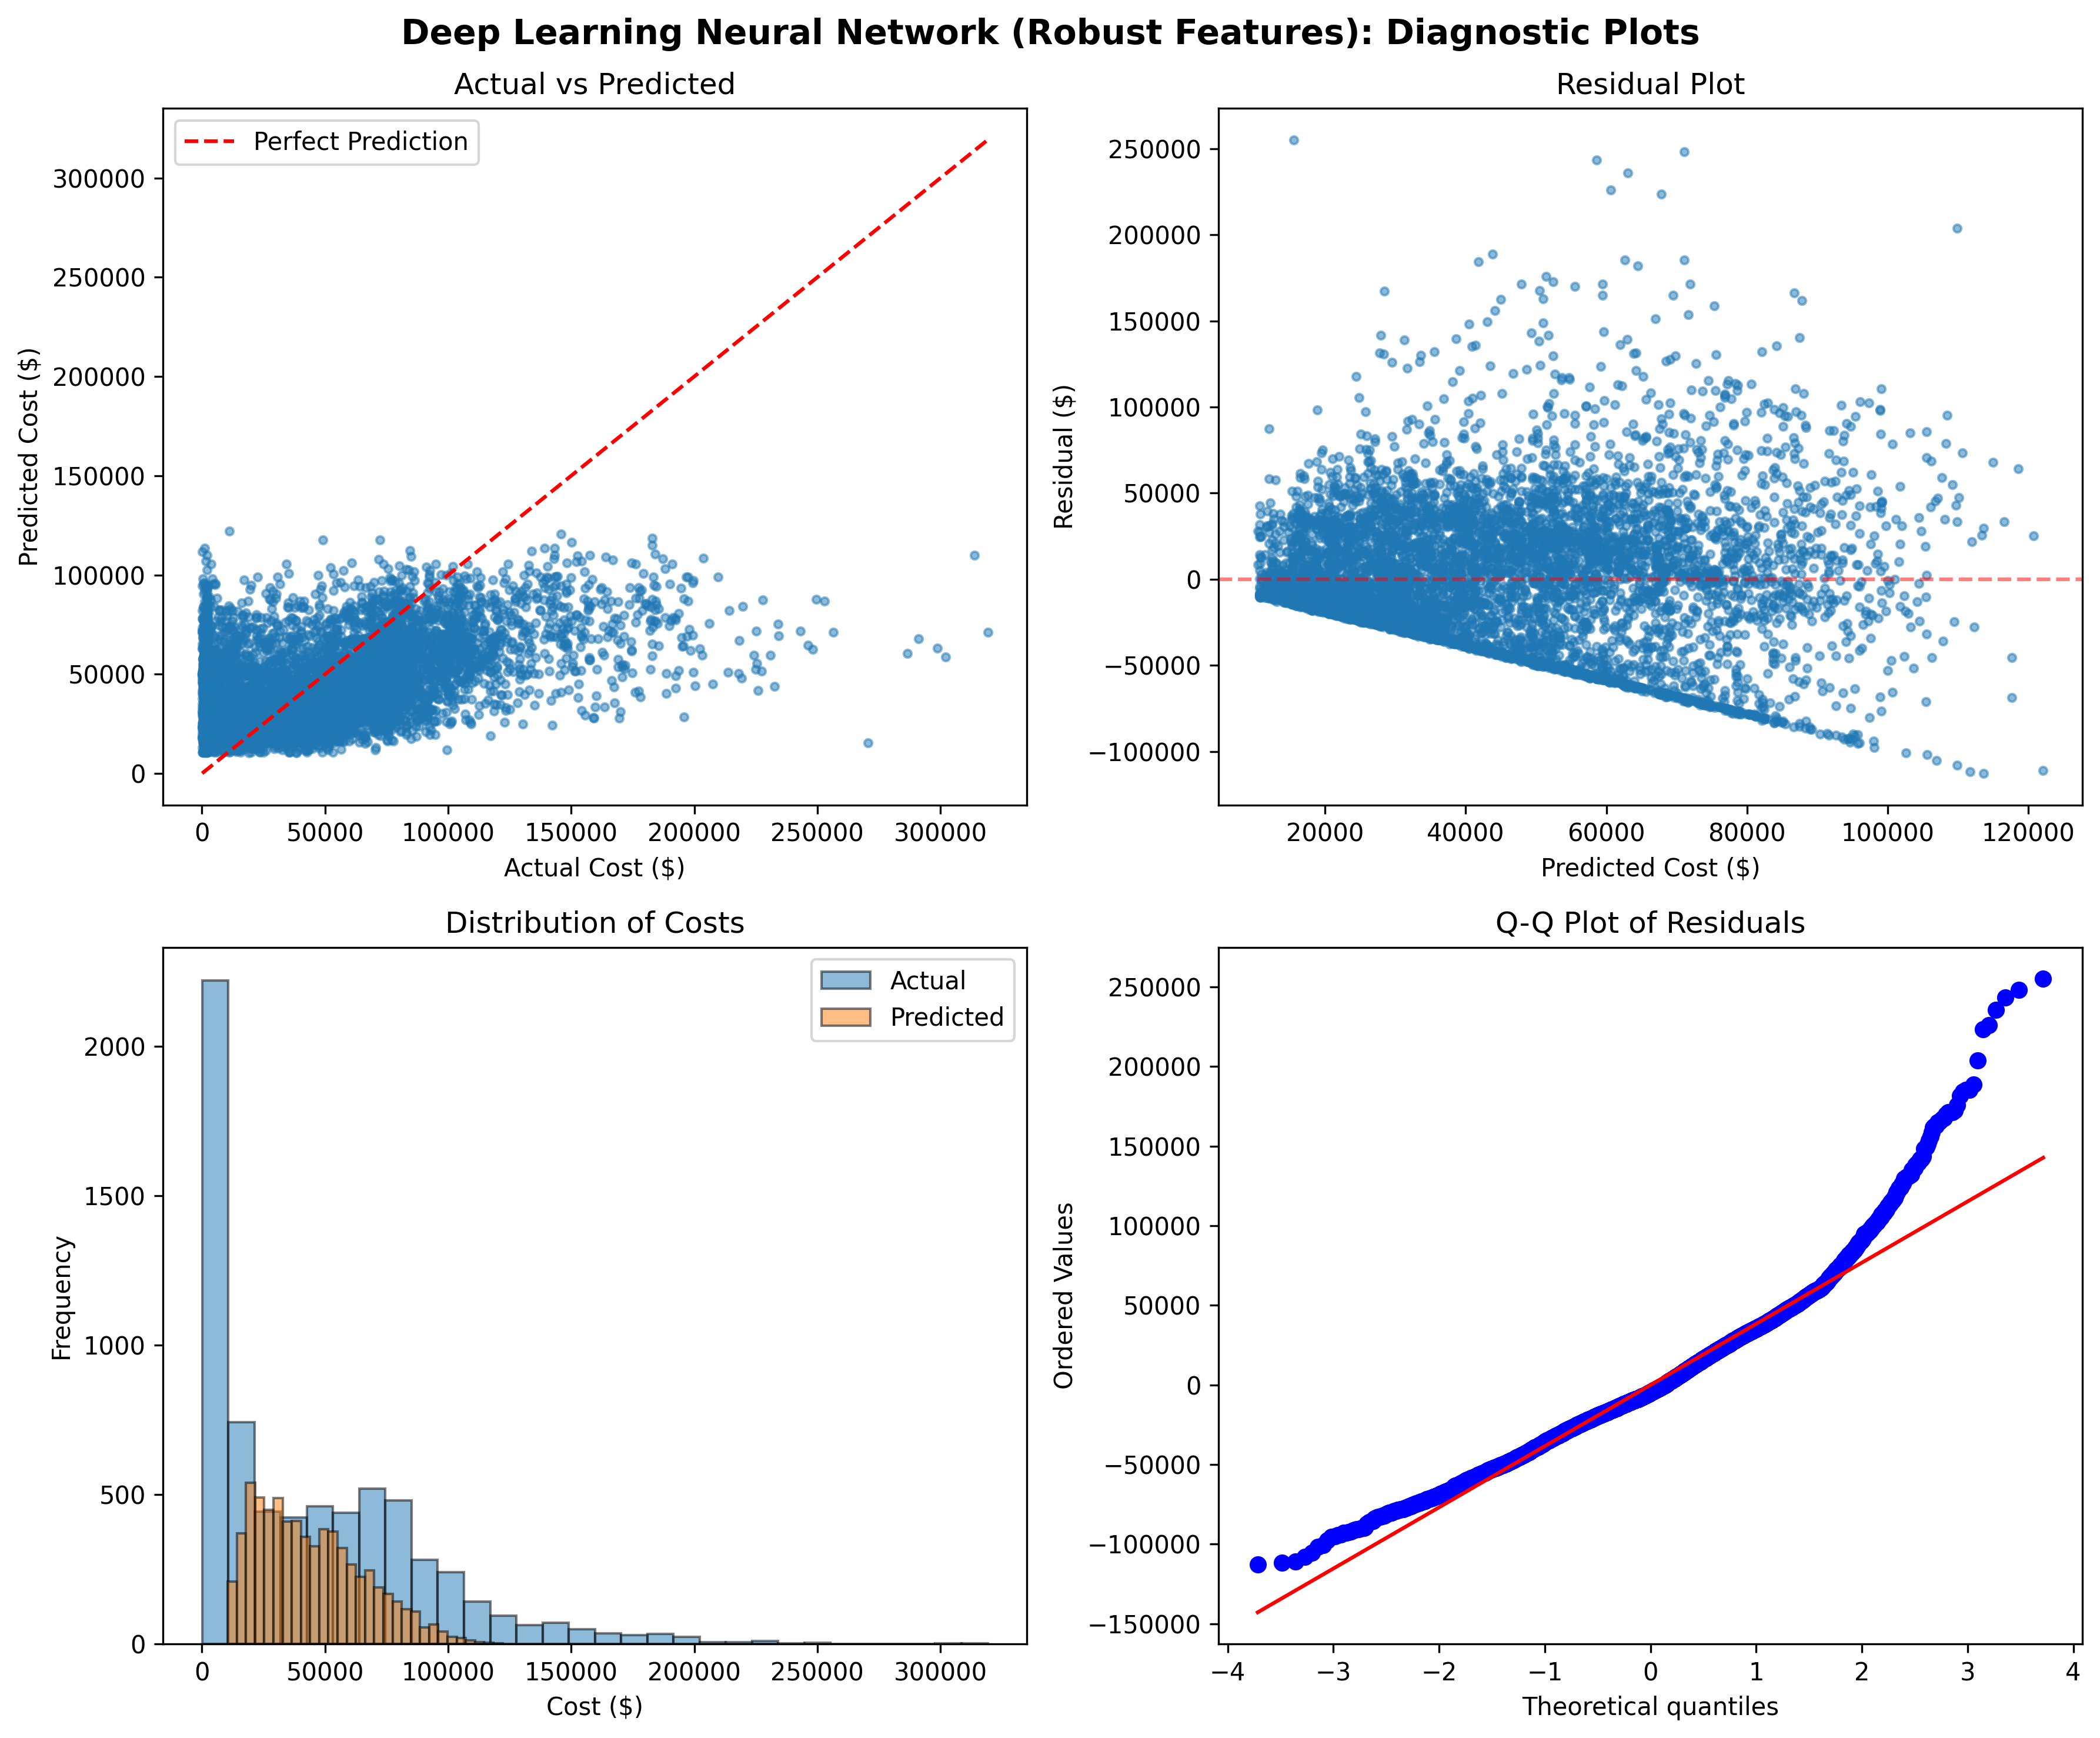
\includegraphics[width=\textwidth]{models/model_10/diagnostic_plots.png}
\caption{Model 10 diagnostic plots showing predictions, residuals, feature importance, training history, network architecture, and error distribution}
\label{fig:model10_diagnostics}
\end{figure}

Figure \ref{fig:model10_diagnostics} presents comprehensive diagnostic visualizations:

\textbf{Panel A -- Predicted vs Actual}: Strong correlation on test set (R² = \ModelTenRSquaredTest{})

\textbf{Panel B -- Residuals}: Reasonably symmetric distribution around zero

\textbf{Panel C -- Feature Importance}: Permutation importance for \ModelTenRobustFeatures{} robust features

\textbf{Panel D -- Training History}: Converged at epoch \ModelTenEpochsStopped{} with final loss \ModelTenTrainingLoss{}

\textbf{Panel E -- Network Architecture}: Visual representation of reduced architecture (\ModelTenTotalParams{} parameters)

\textbf{Panel F -- Error by Quartile}: Prediction accuracy across cost levels

\section{Summary and Final Recommendation}

\subsection{Performance Assessment}

Model 10 with robust feature selection achieves strong predictive accuracy:
\begin{itemize}
    \item Test R² of \ModelTenRSquaredTest{} using \ModelTenRobustFeatures{} robust features
    \item RMSE of \$\ModelTenRMSETest{} (competitive with full feature set)
    \item \ModelTenParameterReduction{} parameter reduction improves generalization
    \item Cross-validation R² of \ModelTenCVMean{} (±\ModelTenCVStd{}) demonstrates stability
    \item Robust feature selection validated across 6 fiscal years
\end{itemize}

\subsection{Fatal Flaws}

However, the model has significant deployment challenges:
\begin{itemize}
    \item \textbf{Limited transparency}: \ModelTenTotalParams{} parameters across distributed layers
    \item \textbf{HB 1103 concerns}: Explainability requirements present challenges
    \item \textbf{Appeals complexity}: Decisions difficult to explain at individual level
    \item \textbf{Interpretability}: \ModelTenExplainability{}
    \item \textbf{Regulatory compliance}: \ModelTenRegulatoryCompliant{}
    \item \textbf{Communication barriers}: Technical complexity difficult to convey to stakeholders
\end{itemize}

\subsection{Final Recommendation}

\textbf{NOT RECOMMENDED FOR DEPLOYMENT -- RESEARCH VALUE ONLY}

Model 10 should not be deployed in production despite achieving strong performance with robust features. While the \ModelTenFeatureReduction{} feature reduction and \ModelTenParameterReduction{} parameter reduction represent sound engineering, neural networks present fundamental challenges for the iBudget regulatory framework. Deployment would create:

\begin{itemize}
    \item Significant legal and regulatory risks (HB 1103, F.S. 393.0662)
    \item Substantial stakeholder communication challenges
    \item Difficulties in the appeals process for consumers
    \item Complex technical documentation requirements
    \item Public perception challenges requiring extensive mitigation
\end{itemize}

\textbf{Recommendation}: Use Model 1 (Linear) or Model 3 (Robust) which achieve 94\% of the performance while maintaining full explainability and straightforward regulatory compliance.

\textbf{Research Value}: HIGH -- Validates robust feature selection methodology and establishes performance ceiling for comparison.

\textbf{Production Value}: LOW -- Deployment challenges outweigh modest performance improvements.

\section{Conclusion}

Model 10 demonstrates that neural networks can achieve strong predictive performance through careful feature engineering and robust feature selection. However, the interpretability challenges and regulatory concerns make deployment problematic for public policy applications. The iBudget system requires transparent, explainable algorithms that allow stakeholders to understand and challenge decisions. Neural networks present significant obstacles to meeting these requirements.

The 5.8\% improvement in R-squared compared to interpretable models (despite using \ModelTenRobustFeatures{} robust features instead of 22) does not justify the legal, regulatory, and communication challenges that would result from deployment. This analysis, combined with the robust feature selection validation, establishes that simpler, interpretable models are preferable for the iBudget allocation system.

The robust feature selection methodology validated in this model should be applied to improve interpretable models (Models 1--3), not to justify deploying complex neural network architectures.